\section{Consensus Protocols}

This section provides background on the consensus protocols that were studied
during the internship in order to evaluate how to integrate this Merkle-tree-based integrity verification protocol into a distributed setting.  
Although corruption detection could be applied in a centralized environment using simple checksums, in a distributed cluster, a consensus algorithm is needed to coordinate nodes and ensure consistent state.  

Several consensus mechanisms were examined, reflecting the long-standing debate between \emph{leader-based} protocols (such as Raft, PBFT, and PB-Raft) and \emph{leaderless} approaches (such as Flutter+Blink). Each design choice has implications for performance, fault tolerance, and implementation complexity.

\subsection{Raft} \label{sec:raft}

Raft \cite{raft} is a consensus protocol designed to be understandable and practical, and it has become widely adopted in distributed systems such as \texttt{etcd} \cite{etcd-raft} and TiKV \cite{tikv-raft}.
It tolerates \emph{crash faults}, but not Byzantine behaviour \cite{lamport1972byzantine}.

Each server on a Raft cluster is modelled as a finite state machine with three possible states:
\begin{itemize}
    \item \textbf{Follower:} Passive state that responds to requests from the leader and candidates.
    \item \textbf{Candidate:} Initiates an election when a follower times out without hearing from a leader.
    \item \textbf{Leader:} Elected through majority vote, responsible for handling client requests and replicating logs.
\end{itemize}

In Figure \ref{fig:raft-participants}, the three server states are illustrated using a finite state machine.

\begin{figure}
    \centering
    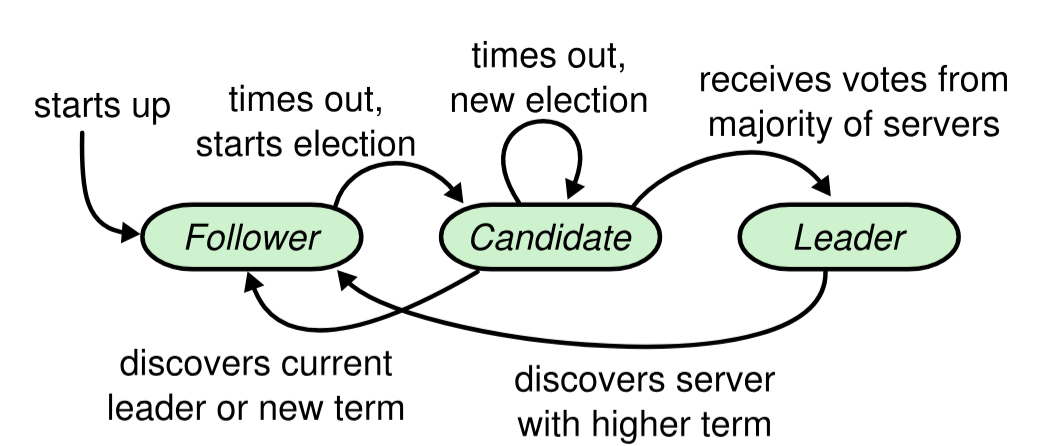
\includegraphics[width=0.7\linewidth]{assets/raft-participants.png}
    \caption{Server states. Followers only respond to requests from other servers. If a follower receives no communication, it becomes a candidate and initiates an election. A candidate that receives votes from a majority of the full cluster becomes the new leader. Leaders typically operate until they fail.}
    \label{fig:raft-participants}
\end{figure}

Leader election in Raft is randomized: followers start an election if they do not receive a heartbeat in a randomized timeout window (e.g., 150--300 ms).  
Candidates send \texttt{RequestVote} messages to all nodes, including their last log index and term, to ensure that outdated nodes cannot become leader.  
If a candidate obtains a majority of votes, it becomes the leader. Otherwise, it retries after another randomized timeout.  

Once elected, the leader replicates client requests in the form of log entries using the \texttt{AppendEntries} message.  
Followers acknowledge receipt and once a majority confirms an entry, it is committed and applied to the state machines.  
This ensures safety (no two servers commit different values at the same log index) and availability (progress can be made as long as a majority of nodes are reachable).

Raft is crash fault-tolerant, but not Byzantine fault-tolerant. However, its simplicity and efficiency make it well-suited for small to medium-sized clusters.

\subsection{Flutter+Blink}

Flutter and Blink \cite{monti2024fast} are Byzantine fault-tolerant protocols that operate without a leader and without cryptographic signatures.  
They require at least $5f+1$ servers to tolerate $f$ Byzantine faults.  

\begin{itemize}
    \item \textbf{Blink:} Provides binary consensus using \emph{Representative Binary Consensus (RBC)}, where a proposal is considered valid only if at least $f+1$ correct servers support it. This in contrast to the single correct server required by Binary Consensus.
    \item \textbf{Flutter:} Builds on Blink to provide total-order broadcast, ensuring all servers agree on the same sequence of client messages.  
    It achieves low latency with a best-case of $2\Delta + \epsilon$, where $\Delta$ is the network delay and $\epsilon$ is negligible.
\end{itemize}

Flutter uses a betting mechanism where clients attach timestamps (bets) to messages. Servers then order messages according to these bets, ensuring global consistency without requiring a centralized leader.  

This makes Flutter+Blink interesting for highly adversarial settings, as they are leaderless, resilient to Byzantine behaviour and even quantum-attack resistant (due to the absence of signatures). However, the $5f+1$ replication requirement can be costly in practice.

\subsection{Practical Byzantine Fault Tolerance (PBFT)}

Practical Byzantine Fault Tolerance (PBFT), introduced by Castro and Liskov in 1999 \cite{castro1999practical}, was the first protocol to show that Byzantine fault tolerance could be practical in asynchronous environments.  
PBFT tolerates up to $f$ Byzantine faults among $3f+1$ replicas, using cryptographic signatures and message authentication codes (MACs) to prevent spoofing and replay attacks.  

The protocol proceeds in three phases:
\begin{enumerate}
    \item \textbf{Pre-prepare:} The leader proposes an order for client requests.
    \item \textbf{Prepare:} Replicas exchange messages to confirm the proposal and ensure consistent ordering.
    \item \textbf{Commit:} Replicas agree to execute the request once a quorum of matching prepare messages is observed.
\end{enumerate}

A client considers its request successful once it receives $f+1$ valid replies. If a timeout occurs, the request is retransmitted.  

PBFT guarantees both safety (no two correct replicas decide differently) and liveness (progress is eventually made under partial synchrony). However, the communication overhead is high: the preparation and committing phases require $O(n^2)$ messages, limiting scalability.  

Despite being somewhat outdated, PBFT remains foundational and continues to inspire more efficient Byzantine consensus protocols.

\subsection{PB-Raft: A Byzantine Extension of Raft}

Raft is widely used due to its simplicity and efficiency, but it only tolerates crash faults. PBFT tolerates Byzantine faults but at a high communication cost.  
PB-Raft \cite{shi2025pb} is a recent proposal that aims to combine the strengths of both.

Key features of PB-Raft include:
\begin{itemize}
    \item \textbf{BLS signatures \cite{boneh2001short}:} Allow short, aggregable multi-signatures that improve efficiency in log replication.
    \item \textbf{PageRank-inspired leader election:} Nodes are ranked by a probability score. Nodes with higher scores use shorter timeouts, balancing fairness and responsiveness.
    \item \textbf{Semi-synchronous model:} Assumes bounded network delays while tolerating Byzantine behaviour.
\end{itemize}

Compared to PBFT, PB-Raft reduces message complexity by adopting Raft's two-phase replication approach while retaining Byzantine resilience.  

\subsection{Summary}

In summary:
\begin{itemize}
    \item \textbf{Raft} is practical, simple and widely adopted for crash fault tolerance.
    \item \textbf{PBFT} provides strong Byzantine fault tolerance but at high communication cost.
    \item \textbf{Flutter+Blink} achieves leaderless, low-latency Byzantine consensus but requires many servers.
    \item \textbf{PB-Raft} is a hybrid approach that adapts Raft for Byzantine environments.
\end{itemize}

For the scope of this thesis, Raft was chosen as the consensus algorithm due to its simplicity, maturity and suitability for a small cluster without Byzantine assumptions.
